\chapter{\textit{Design}}
\chaptermark{\textit{Design}}	%Short version for page header. Comment if not needed
\label{Chapter5}
Neste capitulo será apresentado e descrito o \textit{design} a ser implementado, mencionando também os padrões e princípios que serão usados e recorrendo as várias vistas para representar o sistema graficamente.

\section{Padrões e princípios a serem utilizados}
Para garantir a implementação do sistema como sucesso é fundamental existir a definição de princípios e padrões em antemão à construção do \textit{software} como, por exemplo:
\begin{itemize}
    \item Uso de um \textit{message broker} : Deve ser utilizado um \textit{message broker} para comunicação entre microsserviços
    \item Base de dados por microsserviço: Cada microsserviço deve ter a sua própria base de dados
    \item Escalabilidade horizontal: Projetar o sistema para ser escalável
    \item \textit{Design} orientado a eventos: Deve ser implementado um \textit{design} orientado a eventos
    \item Testes unitários, integração, desempenho e carga: O sistema deve ser testado recorrendo a esses testes
    \item Versões: O uso de \textit{software} de versões é importante, dado as mudanças que pode haver no sistema e caso haja algum impacto negativo por parte de uma nova atualização pode-se sempre voltar para a versão anterior que funcionava sem problemas
    \item Garantia de consistência de dados: Deve ser feita a garantia da consistência de dados 
    \item Modularidade e reuso: O sistema deve ser projetado de uma forma modular permitindo o reuso de componentes 
    \item Padronização de estruturas de dados: Deve ser feita uma definição dos padrões das estruturas de dados compartilhados entre serviços
    \item Documentação clara e atualizada: Para serviço deve ser mantida documentação atualizada e clara
    \item Separação de Responsabilidades: Cada serviço deve ser responsável pelos seus próprios dados
    \item Adoção de objeto de transferência de dados: Devem ser adotados objetos de transferência de dados para o recebimento e envio de dados entre serviços
    \item Uso de \ac{ddd}: Deve ser utilizado o conceito de \textit{DDD} na construção do sistema
    \item Uso de \textit{API Gateway}: A \textit{API Gateway} deve chamar os vários serviços, aumentando desta forma, a segurança do próprio sistema com a implementação de mais uma camada, com esta também é possível aglomerar as informações de todos os serviços num só
\end{itemize}


\section{Conceção arquitetural}
O modelo \textit{"4+1"} é um padrão de \textit{software} que fornece várias perspetivas relativamente ao sistema proposto, sendo que, cada uma foca-se em diferentes aspetos da arquitetura a ser implementada. Este é divido por quatro principais vistas (vista lógica, vista processo, vista de implementação, vista física) e uma adicional (vista de cenários).

\begin{itemize}
    \item Vista lógica: Descreve os componentes do \textit{software}, ou seja, a estrutura interna do sistema
    \item Vista processo: Decompõe o sistema em vários processos e serviços, além disso, descreve como estes se comunicam entre si
    \item Vista de implementação: Descreve como o sistema está organizado nas várias camadas e hierarquias
    \item Vista física: Descreve a distribuição física do sistema e as suas conexões físicas
    \item Vista de cenários: Descreve os vários elementos que pretendem atender as regras de negócio e as várias funcionalidades que o sistema disponibiliza
\end{itemize}

Na figura \ref{fig:c4+1} é apresentada as 5 vistas que o modelo propõem, as referidas anteriormente.

\begin{figure}[H]
    \centering
    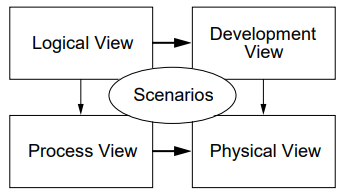
\includegraphics[scale=1]{c4+1.png}
    \caption{Modelo \textit{"4+1"} \cite{c4+1}}
    \label{fig:c4+1}
\end{figure}


\subsection{Vista lógica}

Nas figuras \ref{fig:vistaLogica} e \ref{fig:vistaLogicaBroker} pode-se observar a decomposição do sistema nos vários serviços. O mesmo é divido em seis serviços responsáveis pela logística e um serviço responsável pela deteção de linguagem.

A primeira figura representa um sistema mais primordial, onde a comunicação entre serviços é efetuada por pedidos \textit{HTTP}, o padrão de base de dados por serviço e a \textit{API Gateway} são implementados.

\subsubsection{Diagrama da vista lógica}

\begin{figure}[H]
    \centering
    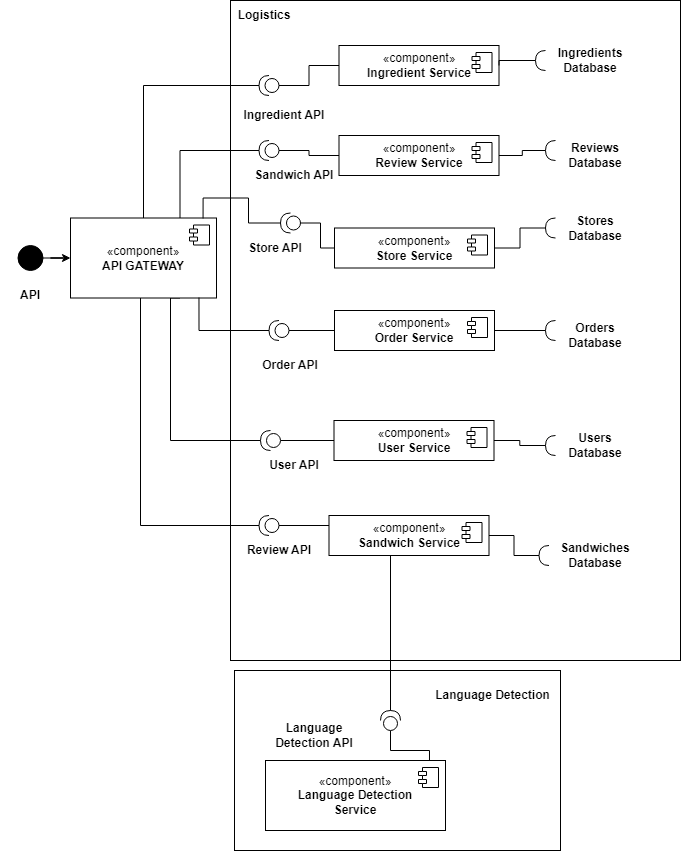
\includegraphics[scale=0.5]{logicalView.png}
    \caption{Diagrama da vista lógica}
    \label{fig:vistaLogica}
\end{figure}

Em comparação à figura \ref{fig:vistaLogica}, a figura \ref{fig:vistaLogicaBroker}, apresenta uma adição na implementação, nesta foi adicionada o \textit{Message Broker}, responsável pelo envio e recebimento de mensagens entre serviços, a troca de destes é realizado através do uso do padrão de \textit{Publish/Subscriber}. O uso deste torna-se importante devido à ineficiência dos pedidos \textit{HTTP} no que diz respeito a desempenho e, por outro lado, torna o processo de escalabilidade horizontal mais simples e eficiente. 

\begin{figure}[H]
    \centering
    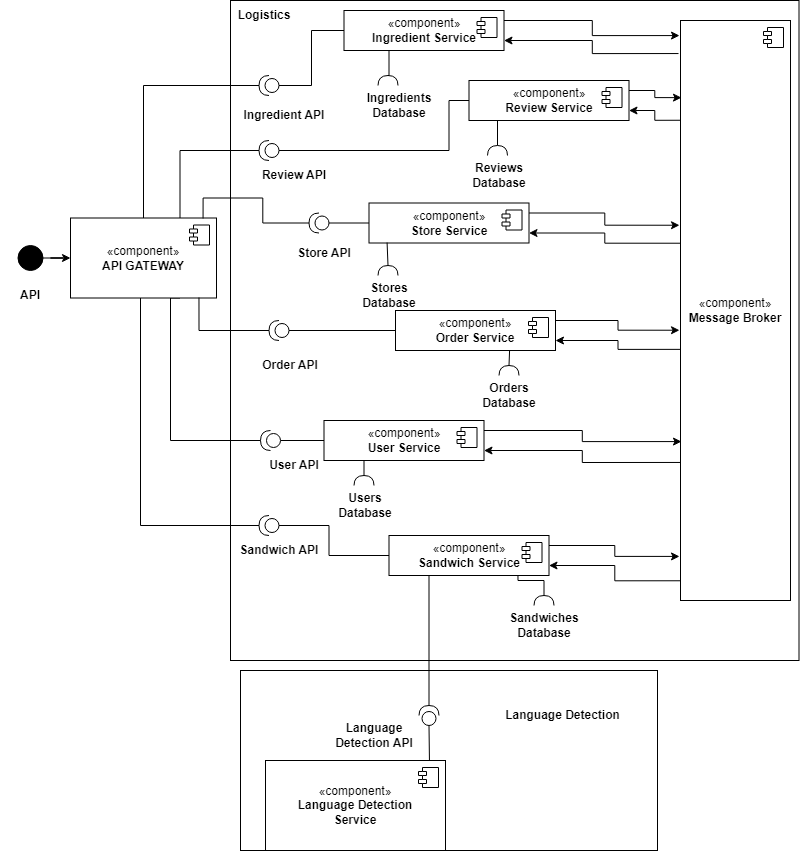
\includegraphics[scale=0.5]{logicalViewWithMessageBroker.png}
    \caption{Diagrama da vista lógica}
    \label{fig:vistaLogicaBroker}
\end{figure}

\subsubsection{Diagrama de Estados}

Um diagrama de estados representa os vários estados ou comportamento, que um certo objeto pode ter ao longo do tempo no sistema. O diagrama a seguir, figura \ref{fig:orderState}, apresenta os possíveis estados de uma encomenda.
Começa com um estado inicial, onde a encomenda é criada e passa para o estado “Criada”. O cliente deverá decidir se contínua com a encomenda ou a cancela até a data da mesma. No caso de a cancelar passa para o estado “Cancelada”, por outro lado, caso o cliente pretenda continuar com a encomenda, então a encomenda é preparada para o processamento, passando para o estado “Em processo”. Após preparada, a encomenda é dada como processada e por isso passa para o estado “Processada”. A partir deste estado, a encomenda está pronta para ser entregue e passa para o estado “Entregue”.

\begin{figure}[H]
    \centering
    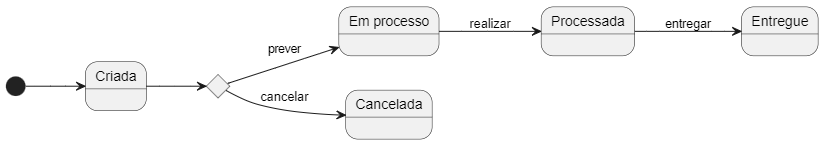
\includegraphics[scale=0.6]{orderState.png}
    \caption{Diagrama de estados para uma encomenda}
    \label{fig:orderState}
\end{figure}

Outro diagrama necessário, figura \ref{fig:reviewState}, é o diagrama de estados para uma crítica, neste é apresentado os possíveis estados para a mesma.
O diagrama começa com a criação da crítica, estado “Criada”. A partir deste estado, o cliente pode realizar a denúncia a uma crítica, levando a um novo estado chamado “Denunciada”. Neste estado, o administrador verificará o conteúdo da mesma, dessa situação pode resultar dois resultados, se a crítica contiver palavras ofensivas é eliminada, o que leva ao estado “Eliminada”, por outro lado, se não contiver nada ofensivo voltará ao estado “Criada”.

\begin{figure}[H]
    \centering
    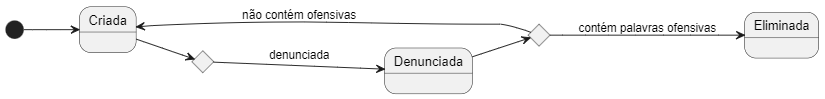
\includegraphics[scale=0.6]{reviewState.png}
    \caption{Diagrama de estados para uma crítica}
    \label{fig:reviewState}
\end{figure}

O diagrama começa com a criação da crítica, estado “Criada”. A partir deste estado, o cliente pode realizar a denúncia a uma crítica, levando a um novo estado chamado “Denunciada”. Neste estado, o administrador verificará o conteúdo da mesma, dessa situação pode resultar dois resultados, se a crítica contiver palavras ofensivas é eliminada, o que leva ao estado “Eliminada”, por outro lado, se não contiver nada ofensivo voltará ao estado “Criada”.

Por último, figura \ref{fig:alterarEstado}, neste diagrama é apresentado os estados que uma sanduíche e um ingrediente podem tomar. O diagrama começa com um estado inicial, estado “Ativo”. A partir deste estado, é possível desativar o ingrediente ou a sanduíche, levando-o ao estado “Inativo”.

A partir do estado "Inativo", é possível reativar o ingrediente ou a sanduíche, levando-o de volta ao estado “Ativo".

\begin{figure}[H]
    \centering
    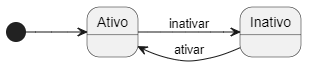
\includegraphics[scale=0.8]{ativarDesativarState.png}
    \caption{Diagrama de estados para uma sanduíche e um ingrediente}
    \label{fig:alterarEstado}
\end{figure}

\subsection{Vista de implementação}

As figuras \ref{fig:implementationView1} e \ref{fig:implementationView2} representam as vistas de implementação nível 1 e nível 2, respetivamente. Com estas figuras é possível perceber-se a relação entre componentes e a estrutura do sistema, no que diz respeito, no contexto da implementação.

Relativamente à figura \ref{fig:implementationView1} é possível observar-se as dependências entre componentes ao nível mais alto, ao nível dos serviços.

\begin{figure}[H]
    \centering
    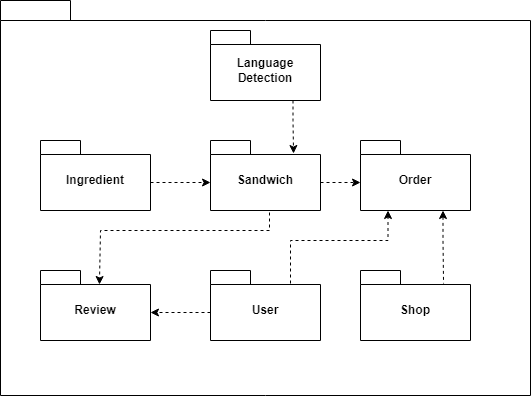
\includegraphics[scale=0.5]{implementationView.png}
    \caption{Diagrama da vista de implementação nível 1}
    \label{fig:implementationView1}
\end{figure}

Agora na figura \ref{fig:implementationView2}, a um nível mais baixo do que na figura anterior, é possível testemunhar a estruturação de um serviço e as suas dependências entre os elementos do próprio serviço. Todos os serviços seguem esta tipologia. Cada serviço é constituído por quatro divisões:
\begin{itemize}
    \item \textit{Controlller}: Ponto de entrada para o serviço e responsável pelo encaminhamento dos pedidos para o \textit{Service}
    \item \textit{Service}: Responsável por toda a lógica do serviço
    \item \textit{Repository}: Responsável pela conexão à base de dados e respetivo manuseamento
    \item \textit{Model}: Responsável por definir os objetos 
\end{itemize}


\begin{figure}[H]
    \centering
    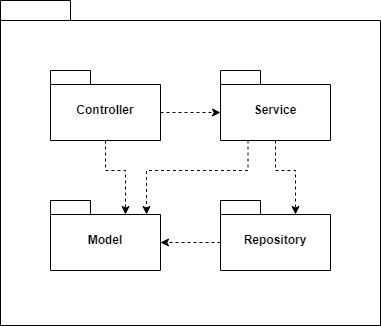
\includegraphics[scale=0.5]{implementationViewLevel2.png}
    \caption{Diagrama da vista de implementação nível 2}
    \label{fig:implementationView2}
\end{figure}

\subsection{Vista de processo}

As seguintes figuras, representam as vistas de processo nível 1 e nível 2, respetivamente. Com estas figuras é possível observar os passos necessários para a conclusão do processo.

A figura \ref{fig:processView1}, representa o processo de criação de um ingrediente ao mais alto nível. O diagrama começa por representar o pedido feito, que será efetuado à \textit{API Gateway}. Posteriormente, este pedido será encaminhado para o serviço correspondente, o que neste caso, será o serviço "Ingredient". Este por sua vez, retornará o ingrediente criado e o código que representa a criação sucedida desse mesmo ingrediente, no caso de haver conflito na autenticação é retornado só o código \textit{HTTP} 403.

\begin{figure}[H]
    \centering
    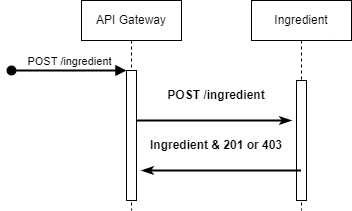
\includegraphics[scale=0.6]{processViewLevel1.png}
    \caption{Diagrama da vista de processo do método \textit{POST} nível 1}
    \label{fig:processView1}
\end{figure}

A figura \ref{fig:processView2}, representa o processo de criação de um ingrediente a um nível mais baixo do que a anterior. O diagrama começa por representar o pedido feito, que será realizado à \textit{API Gateway}. Posteriormente, este pedido será encaminhado para o serviço correspondente, o que neste caso, será o serviço \textit{Ingredient}. Sendo o \textit{IngredientController}, o ponto de partida para o serviço mencionado anteriormente, este é responsável pelo encaminhamento do pedido recebido. A seguir, este chamará a função \textit{createIngredient}, que enviará o objeto introduzido no pedido para o \textit{IngredientService} onde será processado. É neste momento, que será feita a verificação do utilizador, no caso de não lhe ser permitido o acesso, será enviado o código \textit{HTTP} 403, por outro lado, caso se verifique que tem as permissões necessárias, o mesmo objeto mencionado anteriormente, será enviado para o \textit{IngredientRepository}, onde será feito o registo na base de dados criada para o efeito. Já o objeto criado na base de dados é retornado um objeto contendo todos os parâmetros do ingrediente, que terá de passar por um processo de transformação, ou seja, é aplicado o padrão de \textit{software} \textit{DTO}. Com este \textit{DTO} criado será feita uma notificação ao \textit{Message Broker} da sua criação e por último será retornado com o código \textit{HTTP} 201.

\begin{figure}[H]
    \centering
    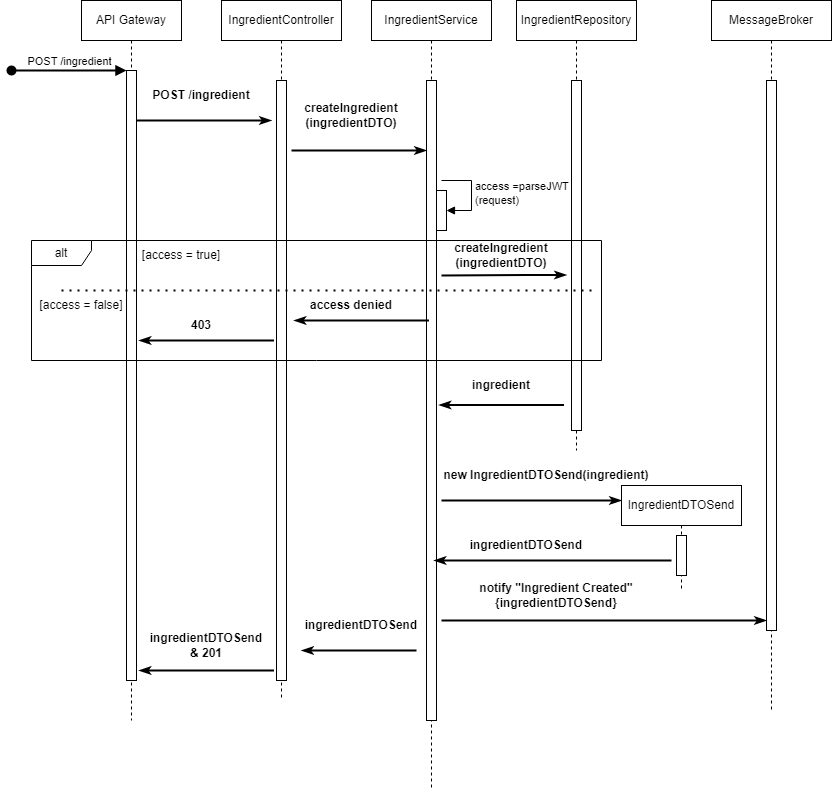
\includegraphics[scale=0.5]{processViewLevel2.png}
    \caption{Diagrama da vista de processo do método \textit{POST} nível 2}
    \label{fig:processView2}
\end{figure}



A figura \ref{fig:processGET1}, representa o processo para obter a lista de todos os ingredientes ao mais alto nível. O diagrama começa por representar o pedido feito, que será efetuado à \textit{API Gateway}. Posteriormente, este pedido será encaminhado para o serviço correspondente, o que neste caso, será o serviço "Ingredient". Este por sua vez, retornará a lista dos ingredientes criados e o código \textit{HTTP} 200.

\begin{figure}[H]
    \centering
    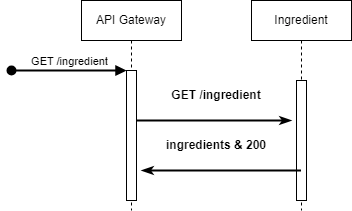
\includegraphics[scale=0.6]{uclevel1_get.png}
    \caption{Diagrama da vista de processo do método \textit{GET} nível 1}
    \label{fig:processGET1}
\end{figure}

A figura \ref{fig:processView2}, representa o processo  para obter a lista de todos os ingredientes a um nível mais baixo do que a anterior. O diagrama começa por representar o pedido feito, que será realizado à \textit{API Gateway}. Posteriormente, este pedido será encaminhado para o serviço correspondente, o que neste caso, será o serviço \textit{Ingredient}. Sendo o \textit{IngredientController}, o ponto de partida para o serviço mencionado anteriormente, este é responsável pelo encaminhamento do pedido recebido. A seguir, este chamará a função \textit{getIngredients}, que pedirá ao \textit{IngredientService} a lista de ingredientes. A seguir, o pedido é reencaminhado para o \textit{IngredientRepository}, onde será feito o pedido à base de dados para esta retornar os ingredientes criados. Já com a lista de ingredientes retornados pela base de dados será necessário passar cada objeto dessa lista para um \textit{DTO} e adicionar esse mesmo a outra lista que será posteriormente retornada, juntamente do código \textit{HTTP} 200.

\begin{figure}[H]
    \centering
    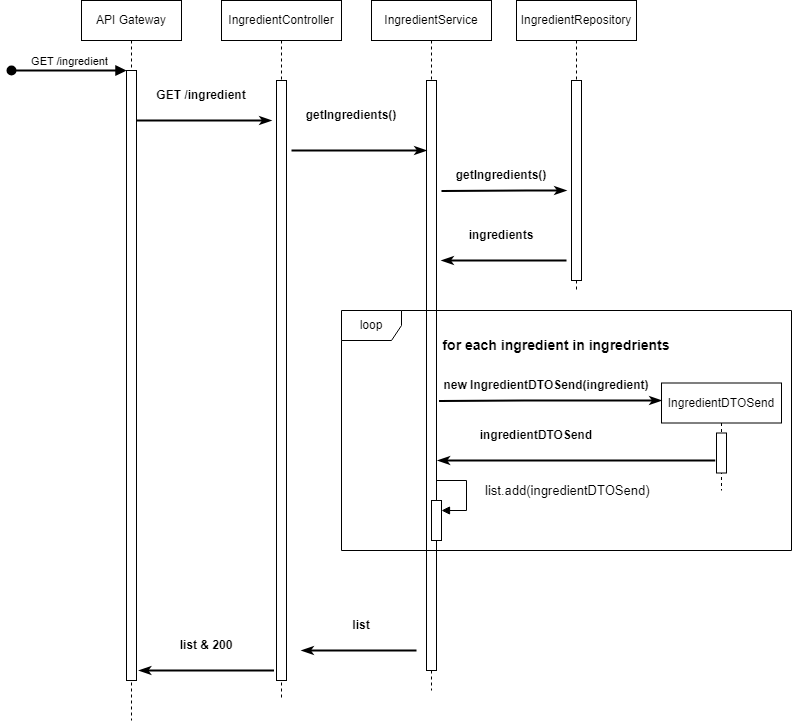
\includegraphics[scale=0.5]{uclevel2_get.png}
    \caption{Diagrama da vista de processo do método \textit{GET} nível 2}
    \label{fig:processGET2}
\end{figure}

A figura \ref{fig:processDELETE1}, representa o processo de eliminação de um ingrediente ao mais alto nível. O diagrama começa por representar o pedido feito, que será efetuado à \textit{API Gateway}. Posteriormente, este pedido será encaminhado para o serviço correspondente, o que neste caso, será o serviço "Ingredient". Este por sua vez, retornará no caso de haver conflito na autenticação o código \textit{HTTP} 403 ou o código \textit{HTTP} 204, se por eliminado com sucesso.


\begin{figure}[H]
    \centering
    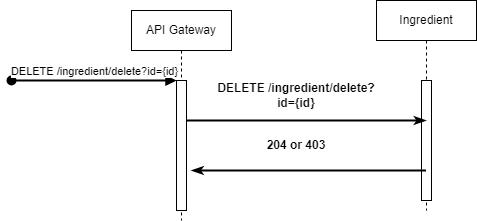
\includegraphics[scale=0.6]{uclevel1_delete.png}
    \caption{Diagrama da vista de processo do método \textit{DELETE} nível 1}
    \label{fig:processDELETE1}
\end{figure}


A figura \ref{fig:processDELETE2}, representa o processo de eliminação de um ingrediente a um nível mais baixo do que a anterior. O diagrama começa por representar o pedido feito, que será realizado à \textit{API Gateway}. Posteriormente, este pedido será encaminhado para o serviço correspondente, o que neste caso, será o serviço \textit{Ingredient}. Sendo o \textit{IngredientController}, o ponto de partida para o serviço mencionado anteriormente, este é responsável pelo encaminhamento do pedido recebido. A seguir, este chamará a função \textit{deleteIngredient}, que enviará o identificador do ingrediente introduzido no pedido para o \textit{IngredientService} onde será processado. É neste momento, que será feita a verificação do utilizador, no caso de não lhe ser permitido o acesso, será enviado o código \textit{HTTP} 403, por outro lado, caso se verifique que tem as permissões necessárias, o mesmo identificador mencionado anteriormente, será enviado para o \textit{IngredientRepository}, onde será feito a eliminação do respetivo ingrediente na base de dados. Já o objeto eliminado na base de dados será feita uma notificação ao \textit{Message Broker} da sua eliminação e por último será retornado com o código \textit{HTTP} 204.

\begin{figure}[H]
    \centering
    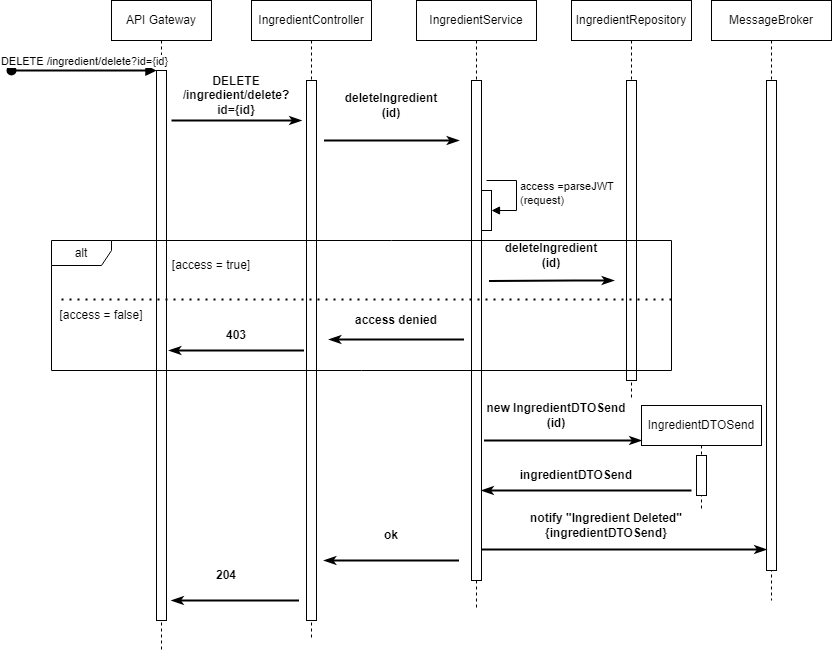
\includegraphics[scale=0.5]{uclevel2_delete.png}
    \caption{Diagrama da vista de processo do método \textit{DELETE} nível 2}
    \label{fig:processDELETE2}
\end{figure}


A figura \ref{fig:processPUT1}, representa o processo de alteração de um ingrediente anteriormente já criado ao mais alto nível. O diagrama começa por representar o pedido feito, que será efetuado à \textit{API Gateway}. Posteriormente, este pedido será encaminhado para o serviço correspondente, o que neste caso, será o serviço "Ingredient". Este por sua vez, retornará o ingrediente alterado e o código que representa a alteração sucedida desse mesmo ingrediente, no caso de haver conflito na autenticação é retornado só o código \textit{HTTP} 403.

\begin{figure}[H]
    \centering
    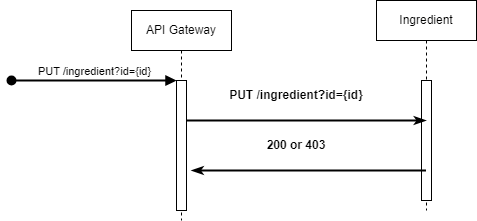
\includegraphics[scale=0.6]{uclevel1_put.png}
    \caption{Diagrama da vista de processo do método \textit{PUT} nível 1}
    \label{fig:processPUT1}
\end{figure}

A figura \ref{fig:processPUT2}, representa o processo de alteração de um ingrediente a um nível mais baixo do que a anterior. O diagrama começa por representar o pedido feito, que será realizado à \textit{API Gateway}. Posteriormente, este pedido será encaminhado para o serviço correspondente, o que neste caso, será o serviço \textit{Ingredient}. Sendo o \textit{IngredientController}, o ponto de partida para o serviço mencionado anteriormente, este é responsável pelo encaminhamento do pedido recebido. A seguir, este chamará a função \textit{updateIngredient}, que enviará o objeto alterado e o identificador introduzido no pedido para o \textit{IngredientService} onde será processado. É neste momento, que será feita a verificação do utilizador, no caso de não lhe ser permitido o acesso, será enviado o código \textit{HTTP} 403, por outro lado, caso se verifique que tem as permissões necessárias, o mesmo objeto mencionado anteriormente, será enviado para o \textit{IngredientRepository}, onde será feito a alteração na base de dados criada para o efeito. Já o objeto alterado na base de dados é retornado um objeto contendo todos os parâmetros do ingrediente, que terá de passar por um processo de transformação, ou seja, é aplicado o padrão de \textit{software} \textit{DTO}. Com este \textit{DTO} criado será feita uma notificação ao \textit{Message Broker} da sua alteração e por último será retornado com o código \textit{HTTP} 201.

\begin{figure}[H]
    \centering
    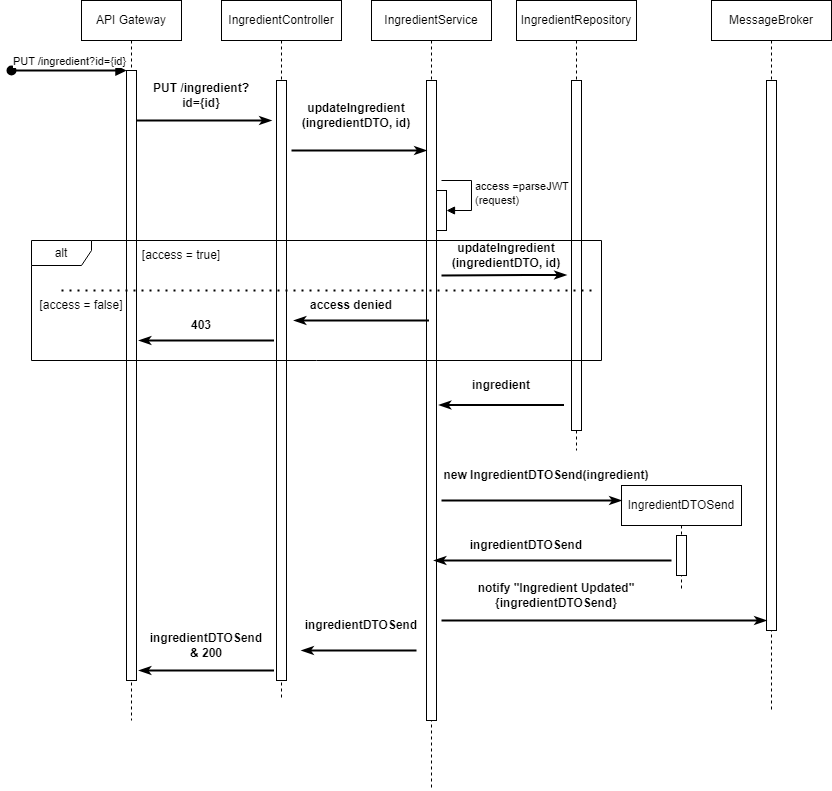
\includegraphics[scale=0.5]{uclevel2_put.png}
    \caption{Diagrama da vista de processo do método \textit{PUT} nível 2}
    \label{fig:processPUT2}
\end{figure}

\subsection{Vista física}

A figura \ref{fig:physicalView} representa a vista física do sistema a ser implementado, ou seja, como está distribuída a infraestrutura do mesmo e como é feita a ligação entre os elementos descritos. A legenda para as linhas destacadas na imagem é:
\begin{itemize}
    \item Linha azul: \textit{MQTT}
    \item Linha vermelho: \textit{HTTP}
    \item Linha amarela: \textit{MySQL Protocol}
\end{itemize}

\begin{figure}[H]
    \centering
    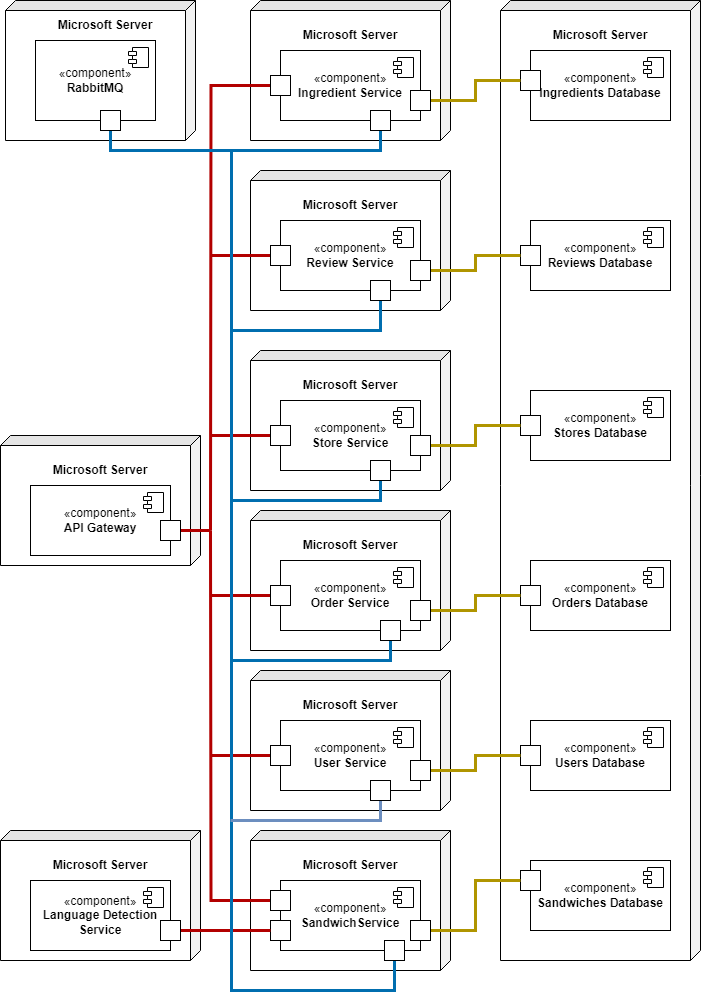
\includegraphics[scale=0.6]{physicalView.png}
    \caption{Diagrama da vista física}
    \label{fig:physicalView}
\end{figure}


\section{Descrição dos microsserviços}

Na seguinte Tabela \ref{table:descricaoMicrosserviços} é feita uma enumeração dos microsserviços a serem desenvolvidos juntamente da sua descrição.

\begin{table}[H]
\caption{Descrição dos microsserviços}
\label{table:descricaoMicrosserviços}
\begin{center}
\begin{tabular}{ |p{5cm}|p{10cm}|  }
\hline
\multicolumn{2}{|c|}{Descrição dos microsserviços} \\
\hline
\textbf{Microsserviço} & \textbf{Descrição} \\
\hline
SandwichService & Disponibiliza funcionalidades para a gestão de sanduíches\\
\hline
IngredientService &  Disponibiliza funcionalidades para a gestão de ingredientes\\
\hline
ReviewService &  Disponibiliza funcionalidades para a gestão de críticas\\
\hline
StoreService &  Disponibiliza funcionalidades para a gestão de lojas\\
\hline
OrderService &  Disponibiliza funcionalidades para a gestão de encomendas\\
\hline
CustomerService &  Disponibiliza funcionalidades para a gestão de clientes\\
\hline
LanguageDectetionService &  Disponibiliza funcionalidades para detetar a linguagem de um certo texto\\
\hline
\end{tabular} 
\end{center}
\end{table}

\section{Diagrama comunicação entre serviços}
Num sistema distribuído, a comunicação entre serviços por muitas vezes é necessária, seja ela efetuada por HTTP ou algum outro método, como, por exemplo, Kafka ou até mesmo RabbitMQ. Dado que, a comunicação síncrona (HTTP) tem problemas como dificuldade de escalabilidade ou a acoplagem de serviços, decidiu-se utilizar a comunicação assíncrona, em concreto o \textit{software} RabbitMQ, dado as suas caraterísticas anteriormente já referidas. O seguinte Figura \ref{fig:modulos} mostra as comunicações que necessitam ser feitas entre serviços.

\begin{figure}[H]
    \centering
    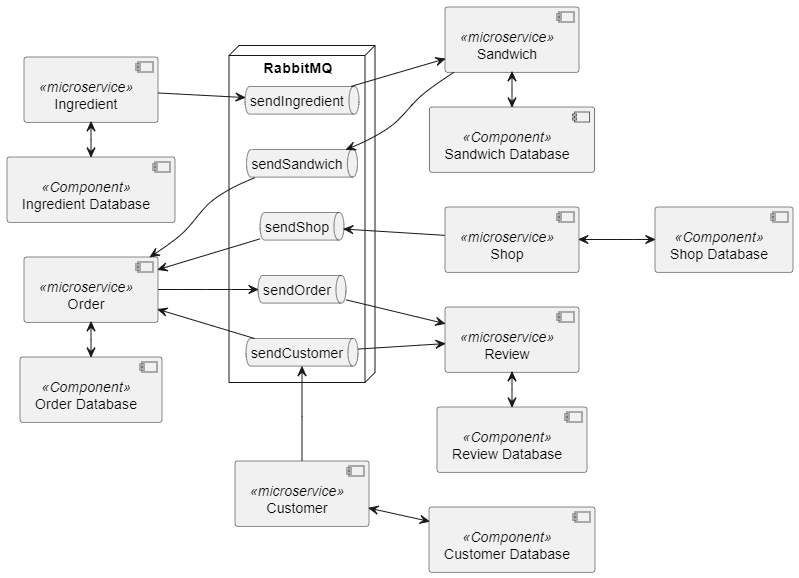
\includegraphics[scale=0.8]{rabbit.png}
    \caption{Diagrama de comunicação entre serviços}
    \label{fig:modulos}
\end{figure}